% \documentclass[9pt,t]{beamer}
\usefonttheme{professionalfonts}
\usefonttheme{serif}
\PassOptionsToPackage{pdfpagemode=FullScreen}{hyperref}
\PassOptionsToPackage{usenames,dvipsnames}{color}
% \DeclareGraphicsRule{*}{mps}{*}{}
\usepackage{linalgjh}
\usepackage{present}
\usepackage{directories}
\usepackage{xr}\externaldocument{\mapdir map2} % read refs from .aux file
\usepackage{xr}\externaldocument{\vsdir vs3} % read refs from .aux file
\usepackage{catchfilebetweentags}
\usepackage{etoolbox} % from http://tex.stackexchange.com/questions/40699/input-only-part-of-a-file-using-catchfilebetweentags-package
\makeatletter
\patchcmd{\CatchFBT@Fin@l}{\endlinechar\m@ne}{}
  {}{\typeout{Unsuccessful patch!}}
\makeatother

\mode<presentation>
{
  \usetheme{boxes}
  \setbeamercovered{invisible}
  \setbeamertemplate{navigation symbols}{} 
}
\addheadbox{filler}{\ }  % create extra space at top of slide 
\hypersetup{colorlinks=true,linkcolor=blue} 

\title[Homomorphisms] % (optional, use only with long paper titles)
{Three.II Homomorphisms}

\author{\textit{Linear Algebra}, edition four \\ {\small Jim Hef{}feron}}
\institute{
  \texttt{https://hefferon.net/linearalgebra}\\[0.25ex]
  \texttt{http://joshua.smcvt.edu/linearalgebra}
}
\date{}


\subject{Homomorphisms}
% This is only inserted into the PDF information catalog. Can be left
% out. 

\begin{document}
\begin{frame}
  \titlepage
\end{frame}

% =============================================
% \begin{frame}{Reduced Echelon Form} 
% \end{frame}



% ..... Three.II.1 .....
\section{Definition}
%..........
\begin{frame}{Homomorphism}
\df[def:Homo]
\ExecuteMetaData[\mapdir map2.tex]{df:Homo}
\end{frame}




%..........
% \begin{frame}
% \ex
% The function $\map{h}{\polyspace_2}{\Re^2}$ given by
% \begin{equation*}
%   h(a+bx+cx^2)
%   =
%   \colvec{a+c \\ 0}
% \end{equation*}
% is a homomorphism. 
% (Note that it is neither one-to-one nor onto.)
% \pause
% Showing that it respects addition is routine.
% \begin{gather*}
%   h(\,(a_1+b_1x+c_1x^2)+(a_2+b_2x+c_2x^2)\,)      \\
%   \begin{align*}
%     \qquad
%     &=h(\,(a_1+a_2)+(b_1+b_2)x+(c_1+c_2)x^2\,)     \\
%     &=\colvec{a_1+a_2+c_1+c_2 \\ 0}                 \\
%     &=\colvec{a_1+c_1 \\ 0}+\colvec{a_2+c_2 \\ 0}   \\
%     &=h(a_1+b_1x+c_1x^2)+h(a_2+b_2x+c_2x^2)       
%   \end{align*}
% \end{gather*}
% \pause
% So is showing that it respects scalar multiplication.
% \begin{equation*}
%   r\cdot h(a+bx+cx^2)
%   =r\cdot\colvec{a+c \\ 0}  
%   =\colvec{ra+rc \\ 0}
%   =h(\,r(a+bx+cx^2)\,)
% \end{equation*}
% \end{frame}



%..........
\begin{frame}
\ex
Of these two maps $\map{h,g}{\Re^2}{\Re}$,
the first is a homomorphism while the second is not.
\begin{equation*}
  \colvec{x \\ y}\mapsunder{h} 2x-3y
  \qquad
  \colvec{x \\ y}\mapsunder{g} 2x-3y+1
\end{equation*}

\pause
The map $h$ respects addition
\begin{multline*}
  h(\colvec{x_1 \\ y_1}+\colvec{x_2 \\ y_2})
  =h(\colvec{x_1+x_2 \\ y_1+y_2})             
  =2(x_1+x_2)-3(y_1+y_2)                    \\
  =(2x_1-3y_1)+(2x_2-3y_2)
  =h(\colvec{x_1 \\ y_1})+h(\colvec{x_2 \\ y_2})
\end{multline*}
and scalar multiplication.
\begin{equation*}
  r\cdot h(\colvec{x \\ y})
  =r\cdot(2x-3y)
  =2rx-3ry
  =(2r)x-(3r)y
  =h(r\cdot\colvec{x \\ y})
\end{equation*}

\pause
In contrast, $g$ does not respect addition.
\begin{equation*} 
  g(\colvec{1 \\ 4}+\colvec{5 \\ 6})=-17
  \qquad
  g(\colvec{1 \\ 4})+g(\colvec{5 \\ 6})=-16
\end{equation*}
\end{frame}




%..........
\begin{frame}
We proved these two while studying isomorphisms.

\lm[le:HomoSendsZeroToZero]\hspace*{-1em}
\ExecuteMetaData[\mapdir map2.tex]{lm:HomoSendsZeroToZero}

\lm[le:HomoPreserveLinCombo]\hspace*{-1em}
\ExecuteMetaData[\mapdir map2.tex]{lm:HomoPreserveLinCombo}

\medskip
To verify that a map is a homomorphism, we most often
use~(2). 

\pause
\ex
Between any two vector spaces the zero map $\map{Z}{V}{W}$ given by
$Z(\vec{v})=\zero_W$ is a linear map.
Using~(2): 
$Z(c_1\vec{v}_1+c_2\vec{v}_2)=\zero_W
   =\zero_W+\zero_W=c_1Z(\vec{v}_1)+c_2Z(\vec{v}_2)$.
\end{frame}




%..........
\begin{frame}
\ex
The \definend{inclusion map} $\map{\iota}{\Re^2}{\Re^3}$
\begin{equation*}
  \iota(\colvec{x  \\ y})
  =\colvec{x \\ y \\ 0}
\end{equation*}
is a homomorphism.
\begin{align*}
  \iota(c_1\cdot\colvec{x_1 \\ y_1}+c_2\cdot\colvec{x_2 \\ y_2})
  &=\iota(\colvec{c_1x_1+c_2x_2 \\ c_1y_1+c_2y_2})       \\
  &=\colvec{c_1x_1+c_2x_2 \\ c_1y_1+c_2y_2 \\ 0}      \\
  &=\colvec{c_1x_1 \\ c_1y_1 \\ 0}
   +\colvec{c_2x_2 \\ c_2y_2 \\ 0}                    \\
  &=c_1\cdot\iota(\colvec{x_1 \\ y_1})+c_2\cdot\iota(\colvec{x_2 \\ y_2})
\end{align*}
\end{frame}




% %..........
% \begin{frame}
% \ex
% Consider 
% this function $\map{h}{\polyspace_1}{\polyspace_1}$.
% \begin{equation*}
%   h(a+bx)=b+bx
% \end{equation*}
% Here are two examples of the action of this function: $1+2x\mapsto 2+2x$
% and $3-x\mapsto-1-x$. 

% \pause
% This is a linear map.
% \begin{multline*}
%   h(\,c_1\cdot (a_1+b_1x)+c_2\cdot(a_2+b_2x)\,)                  \\
%   \begin{aligned}
%     &=h(\,(c_1a_1+c_2a_2)+(c_1b_1+c_2b_2)x\,)       \\
%     &=(c_1b_1+c_2b_2)+(c_1b_1+c_2b_2)x          \\
%     &=(c_1b_1+c_1b_1x)+(c_2b_2+c_2b_2x)         \\
%     &=c_1\cdot h(a_1+b_1x)+c_2\cdot h(a_2+b_2x)
%   \end{aligned}
% \end{multline*}
% \end{frame}




%..........
\begin{frame}
\ex
The derivative is a transformation on polynomial spaces.
For instance, consider
$\map{d/dx}{\polyspace_2}{\polyspace_1}$
given by
\begin{equation*}
  d/dx\,(ax^2+bx+c)=2ax+b
\end{equation*}
(examples are $d/dx\,(3x^2-2x+4)=6x-2$
and $d/dx\,(x^2+1)=2x$).

It is a homomorphism.
\begin{multline*}
  d/dx\,\big(\,r_1(a_1x^2+b_1x+c_1)+r_2(a_2x^2+b_2x+c_2)\,\big)  \hspace*{5em}  \\
  \begin{aligned} 
    &=d/dx\,\big(\,(r_1a_1+r_2a_2)x^2+(r_1b_1+r_2b_2)x+(r_1c_1+r_2c_2)\,\big)   \\
    &=2(r_1a_1+r_2a_2)x+(r_1b_1+r_2b_2)   \\
    &=(2r_1a_1x+r_1b_1)+(2r_2a_2x+r_2b_2)   \\
    &=r_1\cdot d/dx\,(a_1x^2+b_1x+c_1)
      +r_2\cdot d/dx\,(a_2x^2+b_2x+c_2)
  \end{aligned}
\end{multline*}
\end{frame}



% ..........
\begin{frame}
\ex
The \definend{trace} of a square matrix 
is the sum down the upper-left to lower-right diagonal.
Thus
$\map{\trace}{\matspace_{\nbyn{2}}}{\Re}$
is this.
\begin{equation*}
  \trace(\begin{mat}
    a &b \\
    c &d
  \end{mat})
  =a+d
\end{equation*}
It is linear.
\begin{multline*}
  \trace(\,
  r_1\cdot\begin{mat}
    a_1 &b_1 \\
    c_1 &d_1
  \end{mat}
  +
  r_2\cdot\begin{mat}
    a_2 &b_2 \\
    c_2 &d_2
  \end{mat}
  \,)                                              \\
  \begin{aligned}
    &=\trace(
      \begin{mat}
        r_1a_1+r_2a_2 &r_1b_1+r_2b_2 \\
        r_1c_1+r_2c_2 &r_1d_1+r_2d_2
      \end{mat}
      )                                       \\
    &=(r_1a_1+r_2a_2)+(r_1d_1+r_2d_2)         \\
    &=r_1(a_1+d_1)+r_2(a_2+d_2)               \\
    &=r_1\cdot\trace(
      \begin{mat}
        a_1 &b_1 \\
        c_1 &d_1
      \end{mat}
      )
      +
      r_2\cdot\trace(
      \begin{mat}
        a_2 &b_2 \\
        c_2 &d_2
      \end{mat}
      )
  \end{aligned} 
\end{multline*}
\end{frame}



%..........
\begin{frame}
\th[th:HomoDetActOnBasis]
\ExecuteMetaData[\mapdir map2.tex]{th:HomoDetActOnBasis}

  \pause
\iftoggle{showallproofs}{
  \pf
  \ExecuteMetaData[\mapdir map2.tex]{pf:HomoDetActOnBasis0}

  \pause
  \ExecuteMetaData[\mapdir map2.tex]{pf:HomoDetActOnBasis1}
}{
  \ex
  The book has the proof.  
  Here is an illustration.
  Consider a map $\map{h}{\Re^2}{\Re^2}$ with this action on a basis.
  \begin{equation*}
    \colvec{1 \\ 1}\mapsunder{h}\colvec{1 \\ 3}
    \quad
    \colvec{1 \\ 0}\mapsunder{h}\colvec{2 \\ 0}
  \end{equation*}
  The effect of the map on any vector~$\vec{v}$ at all
  is determined by those two facts.
  Represent that vector~$\vec{v}$ with respect to the basis.
  \begin{equation*}
    \colvec{-1 \\ 5}=5\cdot\colvec{1 \\ 1}-6\cdot\colvec{1 \\ 0}
  \end{equation*}
  Compute $h(\vec{v})$ using the definition of homomorphism.
  \begin{equation*}
    h(\vec{v})=h(\,5\cdot\colvec{1 \\ 1}-6\cdot\colvec{1 \\ 0}\,)
    =5\cdot\colvec{1 \\ 3}-6\cdot\colvec{2 \\ 0}
    =\colvec{-7 \\ 15}
  \end{equation*}
}
\end{frame}
\begin{frame}
\iftoggle{showallproofs}{
  \ExecuteMetaData[\mapdir map2.tex]{pf:HomoDetActOnBasis2}
  \qed
}{
  \ex Consider $\map{f}{\Re^3}{\Re^3}$ with this effect on the 
   standard basis.
   \begin{equation*}
     f(\vec{e}_1)=\colvec{1 \\ 2 \\ -1}
     \quad
     f(\vec{e}_2)=\colvec{0 \\ 1 \\ 0}
     \quad
     f(\vec{e}_3)=\colvec{3 \\ -1 \\ 0}
   \end{equation*}
   Because this is the standard basis,
   the effect of the map on any vector $\vec{v}\in\Re^3$ is especially
   easy to compute.
   For instance, 
   \begin{equation*}
     \rep{\colvec{-5 \\ 0 \\ 10}}{\stdbasis_3,\stdbasis_3}
     =\colvec{-5 \\ 0 \\ 10}
   \end{equation*}
   and so we have this.
   \begin{equation*}
     f(\colvec{-5 \\ 0 \\ 10})=-5\cdot\colvec{1 \\ 2 \\ -1}
                               +0\cdot\colvec{0 \\ 1 \\ 0}
                               +10\cdot\colvec{3 \\ -1 \\ 0}
         =\colvec{25 \\ -20 \\ 5}
   \end{equation*}
}

\pause
\df[df:ExtendedLinearly]
\ExecuteMetaData[\mapdir map2.tex]{df:ExtendedLinearly}
\end{frame}




%..........
\begin{frame}
\ex
Consider the action $\map{t_\Theta}{\Re^2}{\Re^2}$ of  
rotating all vectors in the plane through an
angle~$\Theta$.
These drawings show that this map satisfies the addition 
\begin{center}
  \vcenteredhbox{\includegraphics{asy/three_ii_rotate_sum_before.pdf}}
  \qquad$\mapsunder{t_{\pi/6}}$\qquad
  \vcenteredhbox{\includegraphics{asy/three_ii_rotate_sum_after.pdf}}
\end{center}
and scalar multiplication conditions.
\begin{center}
  \vcenteredhbox{\includegraphics{asy/three_ii_rotate_prod_before.pdf}}
  \qquad$\mapsunder{t_{\pi/6}}$\qquad
  \vcenteredhbox{\includegraphics{asy/three_ii_rotate_prod_after.pdf}}
\end{center}
We will develop the formula for $t_\Theta$.
\end{frame}
\begin{frame}
Fix a basis for the domain $\Re^2$; 
the standard basis $\stdbasis_2$ is convenient.
We want the basis vectors mapped as here.
\begin{equation*}
  \vcenteredhbox{\includegraphics{asy/three_ii_rotate_basis.pdf}}
  \qquad
  \colvec{1 \\ 0}\mapsto\colvec[r]{\cos\theta \\ \sin\theta}
  \quad
  \colvec{0 \\ 1}\mapsto\colvec[r]{-\sin\theta \\ \cos\theta}
  % \qquad
  % \vcenteredhbox{\includegraphics{asy/three_ii_rotate.pdf}}
\end{equation*}
\pause
Extend linearly. 
\begin{align*}
  t_{\theta}(\colvec{x \\ y})
  &=
  t_{\theta}(x\cdot\colvec{1 \\ 0}+y\cdot\colvec{0 \\ 1})  \\
  &=
  x\cdot t_{\theta}(\colvec{1 \\ 0})+y\cdot t_{\theta}(\colvec{0 \\ 1})  \\
  &=x\cdot\colvec[r]{\cos\theta \\ \sin\theta}
    +y\cdot\colvec[r]{-\sin\theta \\ \cos\theta}  \\
  &=\colvec{x\cos\theta-y\sin\theta \\ x\sin\theta+y\cos\theta}
\end{align*}
% \pause
% (This map is one-to-one and onto, so it is an automorphism.)
\end{frame}



%..........
\begin{frame}
\ex 
One basis of the space of quadratic polynomials $\polyspace_2$
is $B=\sequence{x^2,x,1}$.
Define  the \definend{evaluation map} 
$\map{\text{eval}_3}{\polyspace_2}{\Re}$ 
by specifying its action on that basis
\begin{equation*}
  x^2\mapsunder{\text{eval}_3}9
  \quad
  x\mapsunder{\text{eval}_3}3
  \quad
  1\mapsunder{\text{eval}_3}1
\end{equation*}
and then extending linearly.
\begin{align*}
  \text{eval}_3(ax^2+bx+c)
   &=a\cdot\text{eval}_3(x^2)
     +b\cdot\text{eval}_3(x)
     +c\cdot\text{eval}_3(1)     \\
   &=9a+3b+c
\end{align*}
For instance,
$\text{eval}_3(x^2+2x+3)=9+6+3=18$.

\pause
On the basis elements, we can describe the action of this map as: 
plugging the value~$3$ in for $x$. 
That remains true when we extend linearly, so
$\text{eval}_3(\,p(x)\,)=p(3)$.
\end{frame}




%..........
\begin{frame}
\df[df:LinearTransformation]
\ExecuteMetaData[\mapdir map2.tex]{df:LinearTransformation}

\pause
\ex
For any vector space $V$ the \definend{identity} map $\map{\textrm{id}}{V}{V}$
given by $\vec{v}\mapsto\vec{v}$ is a linear transformation.
The check is easy.

\pause
\ex
In $\Re^3$ the function $f_{yz}$  
that reflects vectors over the $yz$-plane 
\begin{equation*}
  \colvec{x \\ y \\ z}\mapsunder{f_{yz}}\colvec{-x \\ y \\ z}
\end{equation*}
is a linear
transformation.
\begin{multline*}
  f_{yz}(r_1\colvec{x_1 \\ y_1 \\ z_1}+r_2\colvec{x_2 \\ y_2 \\ z_2})
  =f_{yz}(\colvec{r_1x_1+r_2x_2 \\ r_1y_1+r_2y_2 \\ r_1z_1+r_2z_2})  
  =\colvec{-(r_1x_1+r_2x_2) \\ r_1y_1+r_2y_2 \\ r_1z_1+r_2z_2}    \\
  =r_1\colvec{-x_1 \\ y_1 \\ z_1}+r_2\colvec{-x_2 \\ y_2 \\ z_2}  
  =r_1f_{yz}(\colvec{x_1 \\ y_1 \\ z_1})+r_2f_{yz}(\colvec{x_2 \\ y_2 \\ z_2}) 
\end{multline*}
\end{frame}



%..........
\begin{frame}
\lm[le:SpLinFcns]\hspace*{-1em}
\ExecuteMetaData[\mapdir map2.tex]{lm:SpLinFcns}

\ExecuteMetaData[\mapdir map2.tex]{SpLinFcns}

\iftoggle{showallproofs}{
  \pause
  \pf\hspace*{-1em}
  \ExecuteMetaData[\mapdir map2.tex]{pf:SpLinFcns}
  \qed
}{
  \medskip
  \noindent The book contains the proof; instead 
  we will do a couple of examples.
  \smallskip

  \ex We can combine the two homomorphisms $\map{f,g}{\polyspace_1}{\Re^2}$
  \begin{equation*}
    f(a_0+a_1x)=\colvec{a_0+a_1 \\ 0}
    \qquad
    g(a_0+a_1x)=\colvec{4a_1 \\ a_1}
  \end{equation*}
  into a function $\map{2f+3g}{\polyspace_1}{\Re^2}$
  whose action is this.
  \begin{equation*}
    (2f+3g)\,(a_0+a_1x)=\colvec{2a_0+14a_1 \\ 3a_1}
  \end{equation*}
  The point of the lemma is that the linear combination
  $2f+3g$ is also a homomorphism;
  the check is routine.
  The collection of homomorphisms from $\polyspace_1$ to $\Re^2$
  is closed under linear combinations of those homomorphisms\Dash it 
  is a vector space.
}
\end{frame}
\begin{frame}
\ex
Consider $\linmaps{\Re}{\Re^2}$.
A member of $\linmaps{\Re}{\Re^2}$ is a linear map. 
A linear map is determined by its action on a basis of the domain space.
Fix these bases.
\begin{equation*}
  B_{\Re}=\stdbasis_1=\sequence{1}
  \qquad
  B_{\Re^2}=\stdbasis_2=\sequence{\colvec{1 \\ 0}, 
                                \colvec{0 \\ 1}}
\end{equation*}
Thus the functions that are elements of $\linmaps{\Re}{\Re^2}$
are determined by $c_1$ and $c_2$ here.
\begin{equation*}
  1\mapsunder{t} c_1\colvec{1 \\ 0}+c_2\colvec{0 \\ 1}
\end{equation*}
We could write each such map as $h=h_{c_1,c_2}$.
There are two parameters and thus 
$\linmaps{\Re}{\Re^2}$ is a dimension~$2$ space.
% \pause
% \ex
% Similarly, for $\linmaps{\Re^2}{\Re^3}$, fix
% $\stdbasis_2=\sequence{\vec{e}_1, \vec{e}_2}$ and 
% $\stdbasis_3=\sequence{\textcolor{blue}{\vec{e}_1}, \textcolor{blue}{\vec{e}_2}, \textcolor{blue}{\vec{e}_3}}$
% (note that the blue ones are different; 
% they are three tall).
% We can characterize the elements 
% of $\linmaps{\Re^2}{\Re^3}$ in this way.
% \begin{equation*}
%   \vec{e}_1\mapsunder{t} c_1\textcolor{blue}{\vec{e}_1}+c_2\textcolor{blue}{\vec{e}_2}+c_3\textcolor{blue}{\vec{e}_3}
%   \qquad
%   \vec{e}_2\mapsunder{t} d_1\textcolor{blue}{\vec{e}_1}+d_2\textcolor{blue}{\vec{e}_2}+d_3\textcolor{blue}{\vec{e}_3}
% \end{equation*}
% So, $\linmaps{\Re^2}{\Re^3}$ is six-dimensional.
\end{frame}





% ..... Three.II.2 .....
\section{Range space and null space}
%..........
\begin{frame}
\lm[le:RangeIsSubSp]
\ExecuteMetaData[\mapdir map2.tex]{lm:RangeIsSubSp}

\iftoggle{showallproofs}{
  \pause
  \pf
  \ExecuteMetaData[\mapdir map2.tex]{pf:RangeIsSubSp}
  \qed
}{

  \bigskip
  The book has the proof; we instead consider an example.
}
\end{frame}

\begin{frame}
\ex
Let $\map{f}{\Re^2}{\matspace_{\nbyn{2}}}$ be  
\begin{equation*}
  \colvec{a \\ b}
  \mapsunder{f}
  \begin{mat}
    a  &a+b \\
    2b &b
  \end{mat}
\end{equation*}
(the check that it is a homomorphism is routine).
One subspace of the domain is the $x$~axis.
\begin{equation*}
  S=\set{\colvec{a \\ 0}\suchthat a\in\Re}
\end{equation*}
The image under~$f$ of the $x$~axis is a subspace of 
of the codomain~$\matspace_{\nbyn{2}}$.
\begin{equation*}
  f(S)=\set{
    \begin{mat}
      a &a \\
      0 &0
    \end{mat}
    \suchthat a\in\Re}
\end{equation*}

\pause
Another subspace of $\Re^2$ is $\Re^2$ itself.
The image of $\Re^2$ under $f$ is this subspace of~$\matspace_{\nbyn{2}}$.
\begin{equation*}
  f(\Re^2)=\set{
    \begin{mat}
      1 &1 \\
      0 &0
    \end{mat}\cdot c_1
    +
    \begin{mat}
      0 &1 \\
      2 &1
    \end{mat}\cdot c_2
    \suchthat c_1,c_2\in\Re}
\end{equation*}
\end{frame}
\begin{frame}
\ex
For any angle $\theta$, 
the function $\map{t_{\theta}}{\Re^2}{\Re^2}$ that rotates 
vectors counterclockwise through an angle $\theta$ is a homomorphism.

In the domain~$\Re^2$ each line through the origin is a subspace.
The image of that line under this map is another line through the origin, 
a subspace of the codomain~$\Re^2$. 
\end{frame}


%..........
\begin{frame}{Range space}
\df[df:RangeSpace]
\ExecuteMetaData[\mapdir map2.tex]{df:RangeSpace}

\pause
\ex
This map from $\matspace_{\nbyn{2}}$ to $\Re^2$ is linear.
\begin{equation*}
  \begin{mat}
    a &b \\
    c &d
  \end{mat}
  \mapsunder{h}
  \colvec{a+b  \\ 2a+2b}
\end{equation*}
The range space is a line through the origin.
\begin{equation*}
  \set{\colvec{t \\ 2t} \suchthat t\in\Re}
\end{equation*}
Every member of that set is the image of a $\nbyn{2}$ matrix.
\begin{equation*}
  \colvec{t \\ 2t}
  =
  h(
    \begin{mat}
      t  &0 \\
      0   &0
    \end{mat}
   )
\end{equation*}
The map's rank is $1$.
\end{frame}
\begin{frame}
\ex
The derivative map
$\map{d/dx}{\polyspace_4}{\polyspace_4}$
is linear.
Its range is $\rangespace{d/dx}=\polyspace_3$.
(Verifying that every member of $\polyspace_3$ is the derivative of some 
member of $\polyspace_4$ is easy.)
The rank of this derivative function is the dimension of $\polyspace_3$,
namely~$4$. 

\pause
\ex
Projection $\map{\pi}{\Re^3}{\Re^2}$
\begin{equation*}
  \colvec{x \\ y \\ z}\mapsto\colvec{x \\ y}
\end{equation*}
is a linear map; the check is routine.
The range space is $\rangespace{\pi}=\Re^2$
because given a vector $\vec{w}\in\Re^2$ 
\begin{equation*}
  \vec{w}=\colvec{a \\ b}
\end{equation*}
we can find a
$\vec{v}\in\Re^3$ that maps to it, specifically any $\vec{v}$ with a 
first component~$a$ and second component~$b$.
Thus the rank of $\pi$ is~$2$.

\bigskip\pause
In the book's next section, on computing linear maps,
we will do more examples of determining the range space.
\end{frame}



%..........
\begin{frame}{Many-to-one}
In moving from isomorphisms to homomorphisms we dropped 
the requirement that the maps be onto and one-to-one.
But any homomorphism $\map{h}{V}{W}$ is onto 
its range space $\rangespace{h}$,
so dropping the onto condition has, in a way, no effect
on the range.
It doesn't allow any essentially new maps.

\pause
In contrast,
consider the effect of dropping the one-to-one condition.
With that, an output vector $\vec{w}\in W$
may have many associated inputs,
many $\vec{v}\in V$ such that $h(\vec{v})=\vec{w}$.

\smallskip
\ExecuteMetaData[\mapdir map2.tex]{InverseImage}

\smallskip
The structure of the inverse image sets
will give us insight into the definition of homomorphism.
\end{frame}


\begin{frame}
\ex
Projection $\map{\pi}{\Re^2}{\Re}$ onto the $x$~axis is linear.
\begin{equation*}
  \pi(\,\colvec{x \\ y}\,)
  =x
\end{equation*}
\pause
Here are some elements of $\pi^{-1}(2)$.
Think of these as ``$2$~vectors.''
\begin{center}
  \includegraphics{asy/three_ii_proj_2d01.pdf}
  \qquad\raisebox{0.25in}{$\longmapsto$}\qquad
  \includegraphics{asy/three_ii_proj_2d00.pdf}
\end{center}
Think of elements of $\pi^{-1}(3)$ as ``$3$~vectors.''
\begin{center}
  \includegraphics{asy/three_ii_proj_2d03.pdf}
  \qquad\raisebox{0.25in}{$\longmapsto$}\qquad
  \includegraphics{asy/three_ii_proj_2d02.pdf}
\end{center}
These elements of $\pi^{-1}(5)$ are ``$5$~vectors.''
\begin{center}
  \includegraphics{asy/three_ii_proj_2d05.pdf}
  \qquad\raisebox{0.25in}{$\longmapsto$}\qquad
  \includegraphics{asy/three_ii_proj_2d04.pdf}
\end{center}
\end{frame}
\begin{frame}
These drawings give us a way to make the definition of
homomorphism more concrete.  
Consider preservation of addition.
\begin{equation*}
\pi(\vec{u})+\pi(\vec{v})=\pi(\vec{u}+\vec{v})
\end{equation*}
If $\vec{u}$ is such that  $\pi(\vec{u})=2$,
and $\vec{v}$ is such that $\pi(\vec{v})=3$,
then $\vec{u}+\vec{v}$ will be such that
the sum $\pi(\vec{u}+\vec{v})=5$.
\pause
That is, a ``$2$ vector'' plus a
``$3$~vector'' is a ``$5$~vector.''
Red plus blue makes magenta.
\centergraphic{asy/three_ii_proj_2d06.pdf}

A similar interpretation holds for preservation of scalar multiplication:
the image of an  ``$r\cdot 2$~vector'' is 
$r$ times $2$.
\end{frame}


\begin{frame}
\ex
This function $\map{h}{\Re^2}{\Re^2}$ is linear. 
\begin{equation*}
  \colvec{x \\ y}\mapsto\colvec{x+y \\ 2x+2y}
\end{equation*}
Here are elements of $h^{-1}(\colvec{1 \\ 2})$.
(Only one inverse image element is shown as a vector, most are indicated 
with dots.)
\begin{center}
  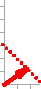
\includegraphics{asy/three_ii_inv_img01.pdf}
  \quad\raisebox{0.25in}{$\longmapsto$}\quad
  
\includegraphics{asy/three_ii_inv_img00.pdf}
\end{center}
Here are some elements of $h^{-1}(\colvec{1.5 \\ 3})$ 
and $h^{-1}(\colvec{2.5 \\ 5})$. 
\begin{center}
  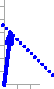
\includegraphics{asy/three_ii_inv_img03.pdf}
  \quad\raisebox{0.25in}{$\longmapsto$}\quad
  
\includegraphics{asy/three_ii_inv_img02.pdf}
  \hspace*{0.75in}
  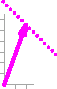
\includegraphics{asy/three_ii_inv_img05.pdf}
  \quad\raisebox{0.25in}{$\longmapsto$}\quad
  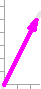
\includegraphics{asy/three_ii_inv_img04.pdf}
\end{center}
\end{frame}
\begin{frame}
The way that the range space vectors add
\begin{equation*}
  {\color{red}\colvec{1 \\ 2}}+{\color{blue}\colvec{1.5 \\ 3}}
   ={\color{magenta}\colvec{2.5 \\ 5}}
\end{equation*}
is reflected in the domain: red plus blue makes magenta. 
\begin{center}
  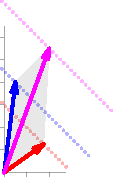
\includegraphics{asy/three_ii_inv_img06.pdf}
\end{center}
\pause
That is, preservation of addition is: 
$h({\color{red}\vec{v}_1})+h({\color{blue}\vec{v}_2})
   =h({\color{magenta}\vec{v}_1+\vec{v}_2})$.
\end{frame}
\begin{frame}{Homomorphisms organize the domain}
So the intuition is that a linear map organizes its domain into inverse 
images, 
\begin{center}  
  \includegraphics{\mapmpdir ch3.5}  % bean to bean; many to one
\end{center}
such that those sets reflect the structure of the range.
\end{frame}



%..........
\begin{frame}
\ex
Projection $\map{\pi}{\Re^3}{\Re^2}$ is a homomorphism.
\begin{equation*}
  \colvec{x \\ y \\ z}\mapsto\colvec{x \\ y}
\end{equation*}
Here we draw the range~$\Re^2$ as the $xy$-plane inside of
$\Re^3$.
\only<1>{\centergraphic{asy/three_ii_3dproj1.pdf}}
\only<2>{\centergraphic{asy/three_ii_3dproj2.pdf}}
\only<3->{\centergraphic{asy/three_ii_3dproj3.pdf}}
In the range the parallelogram shows a vector addition
$\vec{w}_1+\vec{w}_2=\vec{w}_3$.

\pause
\only<2->{The diagram shows some of the  
points in each inverse image~$\pi^{-1}(\vec{w}_1)$, 
$\pi^{-1}(\vec{w}_2)$, and~$\pi^{-1}(\vec{w}_3)$.}
\pause
\only<3->{The sum of a vector $\vec{v}_1\in\pi^{-1}(\vec{w}_1)$ 
and a vector $\vec{v}_2\in\pi^{-1}(\vec{w}_2)$
equals a vector
$\vec{v}_3\in\pi^{-1}(\vec{w}_3)$.
A $\vec{w}_1$ vector plus a
$\vec{w}_2$ vector equals a $\vec{w}_3$ vector.}
\end{frame}




%..........
\begin{frame}
This interpretation of the definition of 
homomorphism also holds when the spaces are not 
ones that we can sketch.

\ex
Let $\map{h}{\polyspace_2}{\Re^2}$ be
\begin{equation*}
  ax^2+bx+c\mapsto\colvec{b \\ b}
\end{equation*}
and consider these three members of the range such that 
$\vec{w}_1+\vec{w}_2=\vec{w}_3$
\begin{equation*}
  \vec{w}_1=\colvec{1 \\ 1}\quad
  \vec{w}_2=\colvec{-1 \\ -1}\quad  
  \vec{w}_3=\colvec{0 \\ 0}
\end{equation*}
\pause
The inverse image of $\vec{w}_1$ is 
$h^{-1}(\vec{w}_1)=\set{a_1x^2+1x+c_1\suchthat a_1,c_1\in\Re^2}$.
% Example members are $3x^2+x+1$, $3x^2+x-4$, and $-2x^2+x$.
Members of this set are ``$\vec{w}_1$~vectors.''
\pause
The inverse image of $\vec{w}_2$ is 
$h^{-1}(\vec{w}_2)=\set{a_2x^2-1x+c_2\suchthat a_2,c_2\in\Re}$;
these are ``$\vec{w}_2$~vectors.''
The ``$\vec{w}_3$~vectors'' are members of
$h^{-1}(\vec{w}_3)=\set{a_3x^2+0x+c_3\suchthat a_3,c_3\in\Re^2}$.

\pause
Any $\vec{v}_1\in h^{-1}(\vec{w}_1)$
plus any $\vec{v}_2\in h^{-1}(\vec{w}_2)$
equals a $\vec{v}_3\in h^{-1}(\vec{w}_3)$:
a quadratic with an $x$~coefficient of $1$ 
plus a quadratic with an $x$~coefficient of $-1$
equals a quadratic with an $x$~coefficient of~$0$.
% \pause
% A ``$\vec{w}_1$~vector'' plus a
% ``$\vec{w}_2$~vector'' is a ``$\vec{w}_3$~vector.'' 
\end{frame}





%..........
\begin{frame}{Null space}
In each of those examples, the homomorphism
$\map{h}{V}{W}$ shows how to view the domain $V$ as organized into the 
inverse images $h^{-1}(\vec{w})$.

In the examples these inverse images are all the same, but shifted.
So if we describe one of them then we understand how the domain is 
divided. 
Vector spaces have a distinguished element, $\vec{0}$.
So we next consider the inverse image $h^{-1}(\zero)$.
\end{frame}


\begin{frame}
\lm[le:NullspIsSubSp]\hspace*{-1em}
\ExecuteMetaData[\mapdir map2.tex]{lm:NullspIsSubSp}


\iftoggle{showallproofs}{
  \pause
  \pf
  \ExecuteMetaData[\mapdir map2.tex]{pf:NullspIsSubSp}
  \qed
}{

  \medskip
  The book has the verification.
}

% \pause
% \medskip
% \no
% This result complements \nearbylemma{le:RangeIsSubSp}%
% that for any subspace of the domain its image is a subspace of the range.
\end{frame}




%..........
\begin{frame}
\df[df:NullSpace]
\ExecuteMetaData[\mapdir map2.tex]{df:NullSpace}

\centergraphic{\mapmpdir ch3.10}
\pause
\no 
Strictly, the trivial subspace of the codomain is not $\zero_{W}$, it is 
$\set{\zero_{W}}$, and
so we may think to write the nullspace as $h^{-1}(\set{\zero_{W}})$.
But we have defined the two sets $h^{-1}(\vec{w})$
and $h^{-1}(\set{\vec{w}})$ to be equal
and the first is easier to write.
\end{frame}




%..........
\begin{frame}
\ex
Consider the derivative $\map{d/dx}{\polyspace_2}{\polyspace_1}$.
This is the nullspace; note that it is a subset of the domain
\begin{equation*}
  \nullspace{d/dx}=\set{ax^2+bx+c \suchthat
                                  2ax+b=0}
\end{equation*}
(the `$0$' there is the zero polynomial $0x+0$).
Now, $2ax+b=0$ if and
only if they have the same constant coefficient 
$b=0$,
the same $x$~coefficient of $a=0$, and the same
coefficient of~$x^2$ (which gives no restriction).
So this is the nullspace, and the nullity is $1$. 
\begin{equation*}
  \nullspace{d/dx}=\set{ax^2+bx+c \suchthat
                                  a=0,\, b=0,\, c\in\Re}
                  =\set{c\suchthat c\in\Re}
\end{equation*}

\ex
The function $\map{h}{\Re^2}{\Re^1}$ given by
\begin{equation*}
  \colvec{a \\ b}\mapsto 2a+b
\end{equation*}
has this null space and so
its nullity is $1$.
\begin{equation*}
  \nullspace{h}
  =\set{\colvec{a \\ b}\suchthat 2a+b=0}
  =\set{\colvec{-1/2 \\ 1}b\suchthat b\in\Re}
\end{equation*}
\end{frame}
\begin{frame}
\ex
The homomorphism $\map{f}{\matspace_{\nbyn{2}}}{\Re^2}$
\begin{equation*}
  \begin{mat}
    a &b \\
    c &d 
  \end{mat}
  \mapsunder{f}
  \colvec{a+b \\ c+d}
\end{equation*}
has this null space
\begin{align*}
  \nullspace{f}
  &=\set{
    \begin{mat}
      a  &b  \\
      c  &d  
    \end{mat}
    \suchthat 
    \text{$a+b=0$ and $c+d=0$}
    }                                 \\
  &=\set{
    \begin{mat}
      -b  &b  \\
      -d  &d
    \end{mat}
    \suchthat
    b,d\in\Re
    }
\end{align*}
and a nullity of $2$.

\ex
The dilation function $\map{d_{3}}{\Re^2}{\Re^2}$
\begin{equation*}
  \colvec{a  \\ b}\mapsto\colvec{3a \\ 3b}
\end{equation*}
has
$\nullspace{d_{3}}=\set{\zero}$.
A trivial space has an empty basis so  $d_{3}$'s nullity is~$0$.
\end{frame}





%..........
\begin{frame}{Rank plus nullity}
Recall the example map $\map{h}{\Re^2}{\Re^2}$
\begin{equation*}
  \colvec{x \\ y}\mapsto\colvec{x+y \\ 2x+2y}
\end{equation*}
whose range space $\rangespace{h}$ is the line $y=2x$
and whose domain is organized into lines, 
$\nullspace{h}$ is the line $y=-x$.
There, an entire line's worth of domain vectors collapses to the
single range point.
\begin{center}
  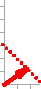
\includegraphics{asy/three_ii_inv_img01.pdf}
  \quad\raisebox{0.25in}{$\longmapsto$}\quad
  
\includegraphics{asy/three_ii_inv_img00.pdf}  
\end{center}
In moving from domain to range, this maps drops a dimension.
We can account for it by thinking that each output point
absorbs a one-dimensional set.
\end{frame}
\begin{frame}
\th[th:RankPlusNullEqDim]
\ExecuteMetaData[\mapdir map2.tex]{th:RankPlusNullEqDim}

\iftoggle{showallproofs}{
  \pause
  \pf
  \ExecuteMetaData[\mapdir map2.tex]{pf:RankPlusNullEqDim0}

  \pause
  \ExecuteMetaData[\mapdir map2.tex]{pf:RankPlusNullEqDim1}

}{

  \medskip
  The book contains the proof.

  \medskip
  \ex Consider this map $\map{h}{\Re^3}{\Re}$.
  \begin{equation*}
    \colvec{x \\ y \\ z}\mapsunder{h} x/2+y/5+z  
  \end{equation*}
  The null space is this plane.
  \begin{equation*}
    \nullspace{h}=
     h^{-1}(0)
     =\set{\colvec{x \\ y \\ z}\suchthat x/2+y/5+z=0}
  \end{equation*}
  Other inverse image sets are also planes.
  \begin{equation*}
     h^{-1}(1)
     =\set{\colvec{x \\ y \\ z}\suchthat x/2+y/5+z=1}
     =\set{\colvec{x \\ y \\ z}\suchthat z=1-x/2-y/5}
  \end{equation*}
}
\end{frame}

\begin{frame}
\iftoggle{showallproofs}{
  \ExecuteMetaData[\mapdir map2.tex]{pf:RankPlusNullEqDim2}
  \qed
}{
  \noindent 
  This shows the inverse images $h^{-1}(0)$ and $h^{-1}(1)$
  lined up on the $z$~axis.
  \begin{center}
    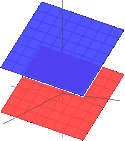
\includegraphics{asy/three_ii_kernel.pdf}
  \end{center}
  So~$h$ breaks the domain into stacked planes\Dash 
  any two inverse images $h^{-1}(r_1)$ and~$h^{-1}(r_2)$ are collections of
  domain vectors whose endpoints form a plane.
  The only difference between these $2$-dimensional subsets
  is where they sit in the stack,
  shown here as where they intersect $z$~axis.

  That is, $h$ partitions the $3$-dimensional domain
  into   
  $2$-dimensional sets, leaving $1$ dimension of
  freedom,
  which matches the dimension of the map's range.
}
\end{frame}


\begin{frame}
\ex
Projection $\map{\pi}{\Re^3}{\Re^2}$ 
\begin{equation*}
  \colvec{a \\ b \\ c}\mapsto\colvec{a \\ b}
\end{equation*}
takes a $3$-dimensional domain
to a $2$-dimensional range.  
Its null space is the $z$-axis, so
its nullity is~$1$.

\pause
This example shows the idea of the proof particularly clearly.
Take 
the basis $B_N=\sequence{\vec{e}_3}$ for the null space. 
\pause
Expand that to the basis $\stdbasis_{3}$ for the entire domain.
\pause
On an input vector the action of $\pi$ is 
\begin{equation*}
  c_1\vec{e}_1+c_2\vec{e}_2+c_3\vec{e}_3
  \quad\mapsto\quad
  c_1\vec{e}_1+c_2\vec{e}_2+\zero
\end{equation*}
and so the domain is organized by~$\pi$ into inverse images 
that are vertical lines, one-dimensional sets 
like the null space.
\centergraphic{asy/three_ii_dims.pdf}
\end{frame}



\begin{frame}
\ex
The derivative function $\map{d/dx}{\polyspace_2}{\polyspace_1}$
\begin{equation*}
  ax^2+bx+c \mapsto 2a\cdot x+b
\end{equation*}
has this range space
\begin{equation*}
  \rangespace{d/dx}=\set{d\cdot x+e\suchthat d, e\in\Re}=\polyspace_{1}
\end{equation*}
(the linear polynomial $dx+e\in\polyspace_{1}$ 
is the image of any antiderivative $(d/2)x^2+ex+C$, where $C\in \Re$).
This is its null space.
\begin{equation*}
  \nullspace{d/dx}=\set{0x^2+0x+c \suchthat c\in\Re}=\set{c \suchthat c\in\Re}
\end{equation*}
The rank is $2$ while the nullity is~$1$, and they add to the domain's 
dimension~$3$.
% \pause
% \ex
% The function $\map{h}{\Re^2}{\Re^1}$ given by
% \begin{equation*}
%   \colvec{a \\ b}\mapsto 2a+b
% \end{equation*}
% has this range space
% \begin{equation*}
%   \rangespace{h}
%   =\set{2a+b\suchthat a,b\in\Re}
%   =\set{c\suchthat c\in\Re}
% \end{equation*}
% and this null space (calculated earlier).
% \begin{equation*}
%   \nullspace{h}
%   =\set{\colvec{-b/2 \\ b}\suchthat b\in\Re}
% \end{equation*}
% Its rank is $1$ and its nullity is $1$.
% Its domain $\Re^2$ has dimension~$2$.
\end{frame}
\begin{frame}
\ex
The dilation function $\map{d_{3}}{\Re^2}{\Re^2}$
\begin{equation*}
  \colvec{a  \\ b}\mapsto\colvec{3a \\ 3b}
\end{equation*}
has range space $\Re^2$
and a trivial nullspace
$\nullspace{d_{3}}=\set{\zero}$.
So its rank is~$2$
and its nullity is~$0$.
% \pause
% \ex
% The homomorphism $\map{f}{\matspace_{\nbyn{2}}}{\Re^2}$
% \begin{equation*}
%   \begin{mat}
%     a &b \\
%     c &d 
%   \end{mat}
%   \mapsunder{f}
%   \colvec{a+b \\ c+d}
% \end{equation*}
% has range space equal to $\Re^2$ (to get a vector with a first component of 
% $x$ and a second component of $y$ we can take $a=x$, $b=0$, $c=y$, and $d=0$).
% Thus $f$'s rank is~$2$.
% We found its null space earlier
% \begin{equation*}
%   \nullspace{f}
%   =\set{
%     \begin{mat}
%       -b  &b  \\
%       -d  &d
%     \end{mat}
%     \suchthat
%     b,d\in\Re
%     }
% \end{equation*}
% and its nullity is $2$.

\pause
\bigskip
The book's next section is on computing linear maps, and
we will compute more null spaces there.
\end{frame}




%..........
\begin{frame}
\lm[lm:ImageLinearlyDependentIsLinearlyDependent]
\ExecuteMetaData[\mapdir map2.tex]{lm:ImageLinearlyDependentIsLinearlyDependent}

\pause
\pf
\ExecuteMetaData[\mapdir map2.tex]{pf:ImageLinearlyDependentIsLinearlyDependent}
\qed

\pause
\ex
The trace function $\map{\trace}{\matspace_{\nbyn{2}}}{\Re}$
\begin{equation*}
  \begin{mat}
    a  &b  \\
    c  &d
  \end{mat}
  \mapsto a+d
\end{equation*}
is linear.
This set of matrices is dependent.
\begin{equation*}
  S=\set{
    \begin{mat}
      1  &0  \\
      0  &0
    \end{mat},\,
    \begin{mat}
      0  &1  \\
      0  &0
    \end{mat},\,
    \begin{mat}
      2  &1  \\
      0  &0
    \end{mat}
    }
\end{equation*}
The three matrices map to $1$, $0$, and $2$ respectively.
The set $\set{1,0,2}\subseteq\Re$ is linearly dependent.
\end{frame}




%..........
\begin{frame}{A one-to-one homomorphism is an isomorphism}
\th[th:OOHomoEquivalence]
\ExecuteMetaData[\mapdir map2.tex]{th:OOHomoEquivalence}

\iftoggle{showallproofs}{
  \pause
  \pf
  \ExecuteMetaData[\mapdir map2.tex]{pf:OOHomoEquivalence0}
}{
  \bigskip
  The book has the proof.
}
\end{frame}
\iftoggle{showallproofs}{
  \begin{frame}
  \ExecuteMetaData[\mapdir map2.tex]{pf:OOHomoEquivalence1}

  \pause
  \ExecuteMetaData[\mapdir map2.tex]{pf:OOHomoEquivalence2}
  \end{frame}
  \begin{frame}
  \ExecuteMetaData[\mapdir map2.tex]{pf:OOHomoEquivalence3}
  \qed
  \end{frame}
}{}






% ..... Three.II.1 .....
\section{Transformations of $\Re^2$}
%..........
\begin{frame}{Lines go to lines}
In a real space $\Re^n$ a line through the origin is a set 
$\set{r\cdot \vec{v}\suchthat r\in\Re}$ of multiples of a 
nonzero vector. 

Consider a transformation
$\map{t}{\Re^n}{\Re^n}$.
% A defining property of linear maps is that 
% $t(r\cdot\vec{v})=r\cdot t(\vec{v})$.
It is linear and so $t$'s action 
\begin{equation*}
  r\cdot\vec{v}\mapsunder{t} r\cdot t(\vec{v})
\end{equation*}
sends members of the line $\set{r\cdot \vec{v}\suchthat r\in\Re}$
in the domain to members of the line
$\set{s\cdot t(\vec{v})\suchthat s\in\Re}$
in the codomain. 

Thus, under a transformation, lines through the origin 
map to lines through the origin.
Further, the action of~$t$ is determined by its effect $t(\vec{v})$
on any nonzero element of the domain line.
\end{frame}
\begin{frame}
\ex
Consider the line~$y=2x$ in the plane 
\begin{equation*}
  \set{r\cdot\colvec{1 \\ 2}\suchthat r\in\Re}
\end{equation*}
and this transformation.
\begin{equation*}
  \colvec{x \\ y}
  \mapsto
  \colvec{x+3y \\ 2x+4y}
\end{equation*}
The map's effect on any vector in the line is easy to compute.
\begin{equation*}
  \vec{v}=\colvec{1 \\ 2}\mapsunder{t}\colvec{7 \\ 10}
\end{equation*}
The linear map property 
$t(r\cdot\vec{v})=r\cdot t(\vec{v})$
imposes a uniformity on $t$'s action:~$t$ 
has twice the effect on $2\vec{v}$, three times the
effect on $3\vec{v}$, etc.
\begin{equation*}
  \colvec{2 \\ 4}\mapsunder{t}\colvec{14 \\ 20}
  \qquad
  \colvec{-3 \\ -6}\mapsunder{t}\colvec{-21 \\ -30}
  \qquad
  \colvec{r \\ 2r}\mapsunder{t}\colvec{7r \\ 10r}
\end{equation*}
In short: the action of $t$ on any  nonzero $\vec{v}$
determines its action on any other vector $r\vec{v}$
in the line $\spanof{\set{\vec{v}}}$.
\end{frame}


\begin{frame}
  \frametitle{Pick one, any one}
Every plane vector is in some line through the origin
so to understand what $\map{t}{\Re^2}{\Re^2}$ does 
to plane elements it suffices to 
understand what it does to lines through the origin. 
\pause
By the prior slide, to understand what $t$ does to a line through the 
origin it suffices to understand what it does to a single nonzero
vector in that line.

\pause
So one way to understand a transformation's action is to take
a set containing one nonzero vector from each line through the origin,
and describe where the transformation maps the elements of that set.

A natural set with one nonzero element from each line through the
origin is the upper half unit circle (we will explain the colors below).
\begin{equation*}
  \set{\colvec{x \\ y}
       =\colvec{\cos(t) \\ \sin(t)}
         \suchthat 
         0\leq t<\pi}
  \qquad
  \vcenteredhbox{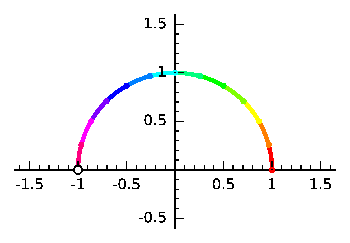
\includegraphics[scale=.75]{graphics/three_ii_a_unithalfcircle.pdf}}  
\end{equation*}  
\end{frame}


\begin{frame}{Dilate $x$}
\ex
The map
\begin{equation*}
  \colvec{x \\ y} \mapsto \colvec{2x \\ y}
\end{equation*}
doubles the first coordinate while keeping the second coordinate constant.
This shows the transformation of the upper half circle.
\begin{equation*}
  \vcenteredhbox{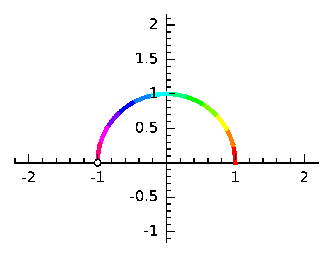
\includegraphics[scale=.75]{graphics/three_ii_a_dialatex1.pdf}}
  \quad\rightarrow\quad
  \vcenteredhbox{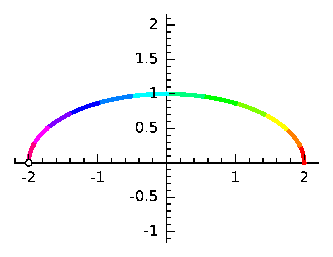
\includegraphics[scale=.75]{graphics/three_ii_a_dialatex2.pdf}}
\end{equation*}
\end{frame}


\begin{frame}{Reverse orientation}
\ex
Here we dilate by a negative.
\begin{equation*}
  \colvec{x \\ y} \mapsto \colvec{-x \\ y}
\end{equation*}
The transformation of the upper half circle
shows why we used the colors.
In the domain they are, taken counterclockwise, red, orange, yellow,
green, blue, indigo, violet.
In the codomain, again taken counterclockwise, they do the opposite. 
\begin{equation*}
  \vcenteredhbox{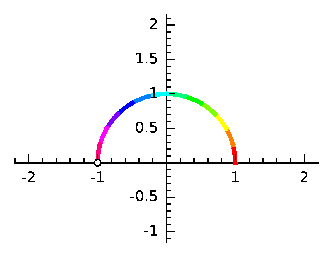
\includegraphics[scale=.75]{graphics/three_ii_a_reversex1.pdf}}
  \quad\rightarrow\quad
  \vcenteredhbox{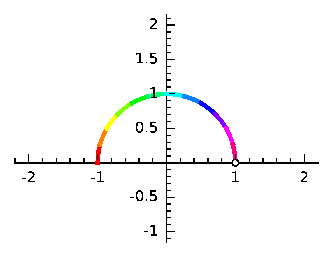
\includegraphics[scale=.75]{graphics/three_ii_a_reversex2.pdf}}
\end{equation*}
\end{frame}


\begin{frame}{Combine dilations}
\ex
Here we dilate both $x$ and~$y$.
\begin{equation*}
  \colvec{x \\ y} \mapsto \colvec{-x \\ 3y}
\end{equation*}
Again the color order reverses, in addition to the stretching 
along the $y$~axis.
\begin{equation*}
  \vcenteredhbox{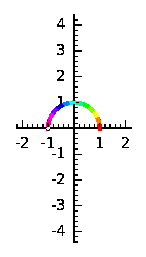
\includegraphics[scale=.75]{graphics/three_ii_a_diagmap1.pdf}}
  \quad\rightarrow\quad
  \vcenteredhbox{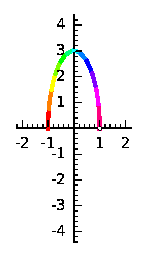
\includegraphics[scale=.75]{graphics/three_ii_a_diagmap2.pdf}}
\end{equation*}
The two dilations 
combine independently in that the first coordinate of the output uses 
only~$x$ and the second coordinate of the output uses only~$y$. 
\end{frame}


\begin{frame}{Skew}
\ex
Next is a map with an output coordinate affected by both $x$ and~$y$.
\begin{equation*}
  \colvec{x \\ y} \mapsto \colvec{x+2y \\ y}
\end{equation*}
\begin{equation*}
  \vcenteredhbox{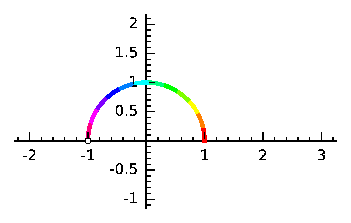
\includegraphics[scale=.75]{graphics/three_ii_a_skew1.pdf}}
  \quad\rightarrow\quad
  \vcenteredhbox{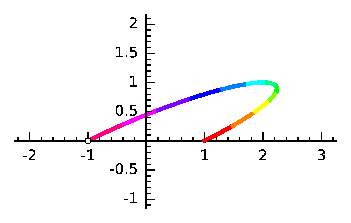
\includegraphics[scale=.75]{graphics/three_ii_a_skew2.pdf}}
\end{equation*}
On the $x$~axis, where~$y=0$, the output's first coordinate is the 
same as the input's first coordinate.
However as we move away from the $x$~axis the $y$'s get larger, and the 
first coordinate of the output is increasingly affected.
(One definition of \textit{skew} is:~having an oblique direction or 
position; slanting.)
\end{frame}


\begin{frame}{Skew the other way}
\ex
We can flip which output coordinate is affected by both $x$ and~$y$.
\begin{equation*}
  \colvec{x \\ y} \mapsto \colvec{x \\ 2x+y}
\end{equation*}
\begin{equation*}
  \vcenteredhbox{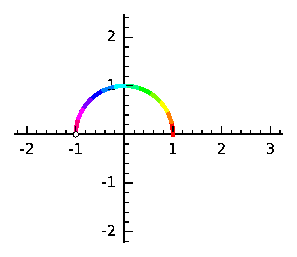
\includegraphics[scale=.75]{graphics/three_ii_a_changeskew1.pdf}}
  \quad\rightarrow\quad
  \vcenteredhbox{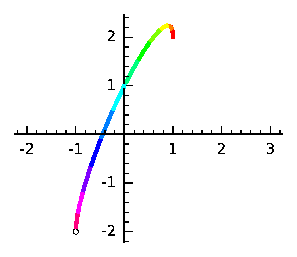
\includegraphics[scale=.75]{graphics/three_ii_a_changeskew2.pdf}}
\end{equation*}
In addition to dilation 
we see clear rotation, for instance of 
the red input vector. 
\end{frame}


\begin{frame}{Same idea but with a smaller effect}
\ex
\begin{equation*}
  \colvec{x \\ y} \mapsto \colvec{x \\ (1/2)x+y}
\end{equation*}
\begin{equation*}
  \vcenteredhbox{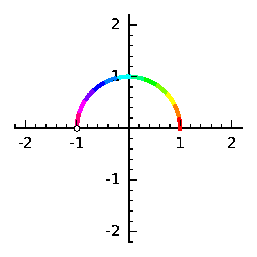
\includegraphics[scale=.75]{graphics/three_ii_a_otherskew1.pdf}}
  \quad\rightarrow\quad
  \vcenteredhbox{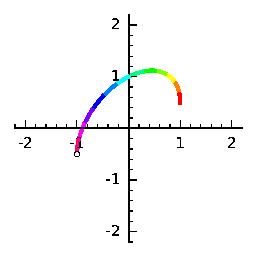
\includegraphics[scale=.75]{graphics/three_ii_a_otherskew2.pdf}}
\end{equation*}
Observe that the rotation is not even.  
A red vector is rotated quite a bit but a green vector, near the
$y$~axis, is not rotated much.
And right on the $y$-axis the vector is not rotated at all. 
\end{frame}


\begin{frame}{Pure roation}
\ex
This rotates every vector counterclockwise through the angle~$\theta$. 
\begin{equation*} 
  \colvec{x \\ y} \mapsto \colvec{\cos(\theta)\cdot x-\sin(\theta)\cdot y \\ \cos(\theta)\cdot x+\sin(\theta)\cdot y} 
\end{equation*}
In this picture $\theta=\pi/6$.
\begin{equation*}
  \vcenteredhbox{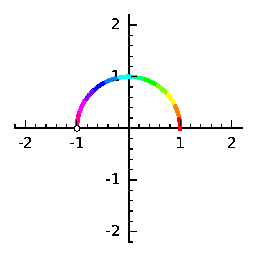
\includegraphics[scale=.75]{graphics/three_ii_a_rotation1.pdf}}
  \quad\rightarrow\quad
  \vcenteredhbox{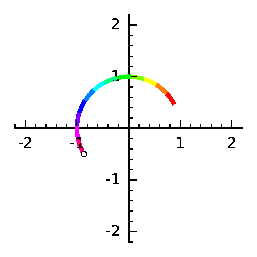
\includegraphics[scale=.75]{graphics/three_ii_a_rotation2.pdf}}
\end{equation*}
\end{frame}


\begin{frame}{Projection}
\ex
Maps can lose a dimension. 
\begin{equation*} 
  \colvec{x \\ y} \mapsto \colvec{x \\ 0}
\end{equation*}
The output is one-dimensional.
\begin{equation*}
  \vcenteredhbox{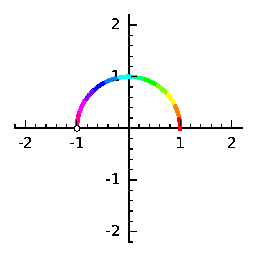
\includegraphics[scale=.75]{graphics/three_ii_a_projection1.pdf}}
  \quad\rightarrow\quad
  \vcenteredhbox{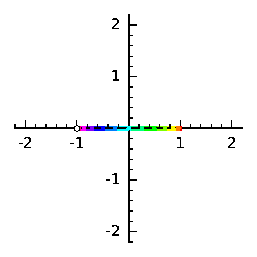
\includegraphics[scale=.75]{graphics/three_ii_a_projection2.pdf}}
\end{equation*}
\end{frame}


\begin{frame}
\ex
The map may project the input vector to a line that is not an axis.
\begin{equation*} 
  \colvec{x \\ y} \mapsto \colvec{x \\ 2x}
\end{equation*}
The two-dimensional input is sent to an output that is one-dimensional.
\begin{equation*}
  \vcenteredhbox{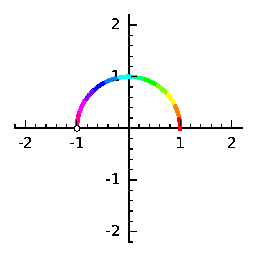
\includegraphics[scale=.75]{graphics/three_ii_a_otherprojection1.pdf}}
  \quad\rightarrow\quad
  \vcenteredhbox{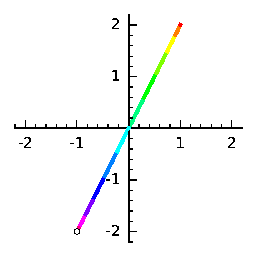
\includegraphics[scale=.75]{graphics/three_ii_a_otherprojection2.pdf}}
\end{equation*}
\end{frame}


\begin{frame}{A generic map}
\ex
An arbitrary map 
\begin{equation*} 
  \colvec{x \\ y} \mapsto \colvec{x+2y \\ 3x+4y}
\end{equation*}
may have an action that is a mixture of the effects shown above.
\begin{equation*}
  \vcenteredhbox{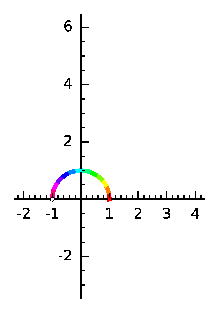
\includegraphics[scale=.75]{graphics/three_ii_a_generic1.pdf}}
  \quad\rightarrow\quad
  \vcenteredhbox{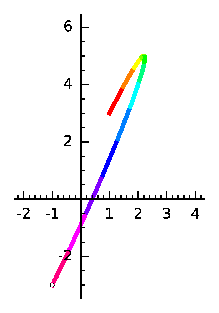
\includegraphics[scale=.75]{graphics/three_ii_a_generic2.pdf}}
\end{equation*}
This shows dilation, rotation, and orientation reversal.
\end{frame}




%...........................
% \begin{frame}
% \ExecuteMetaData[../gr3.tex]{GaussJordanReduction}
% \df[def:RedEchForm]
% 
% \end{frame}
\end{document}
